
\chapter{Detector Layout and Technologies}




\section{Overall structure of the detector}
\writer{Claude Vallee, Karsten Buesser}{1}

The geometrical structure of the ILD detector and the individual layouts of subdetectors were described in details in the ILD LOI [ref] and DBD [ref]. This section shortly reminds the main characteristics with emphasis on the recent evolutions and open options. The main design changes implemented since the DBD take into account continuous progress in detector technology R\&D and the new optics of the ILC interaction region (chapter 3). In the following all dimensions are given for the large version of the detector (see section 4.2 for reduction factors of the small ILD).

\vspace{2cm}

\subsection{Global structure and parameters}
\writer{Claude Vallee, Karsten Buesser}{1}

%\textit{Reminder of the global structure of the ILD detector, focusing details on the main changes since DBD, and mentioning remaining open options like anti-DID.}

\begin{figure}[t!]
\centering
%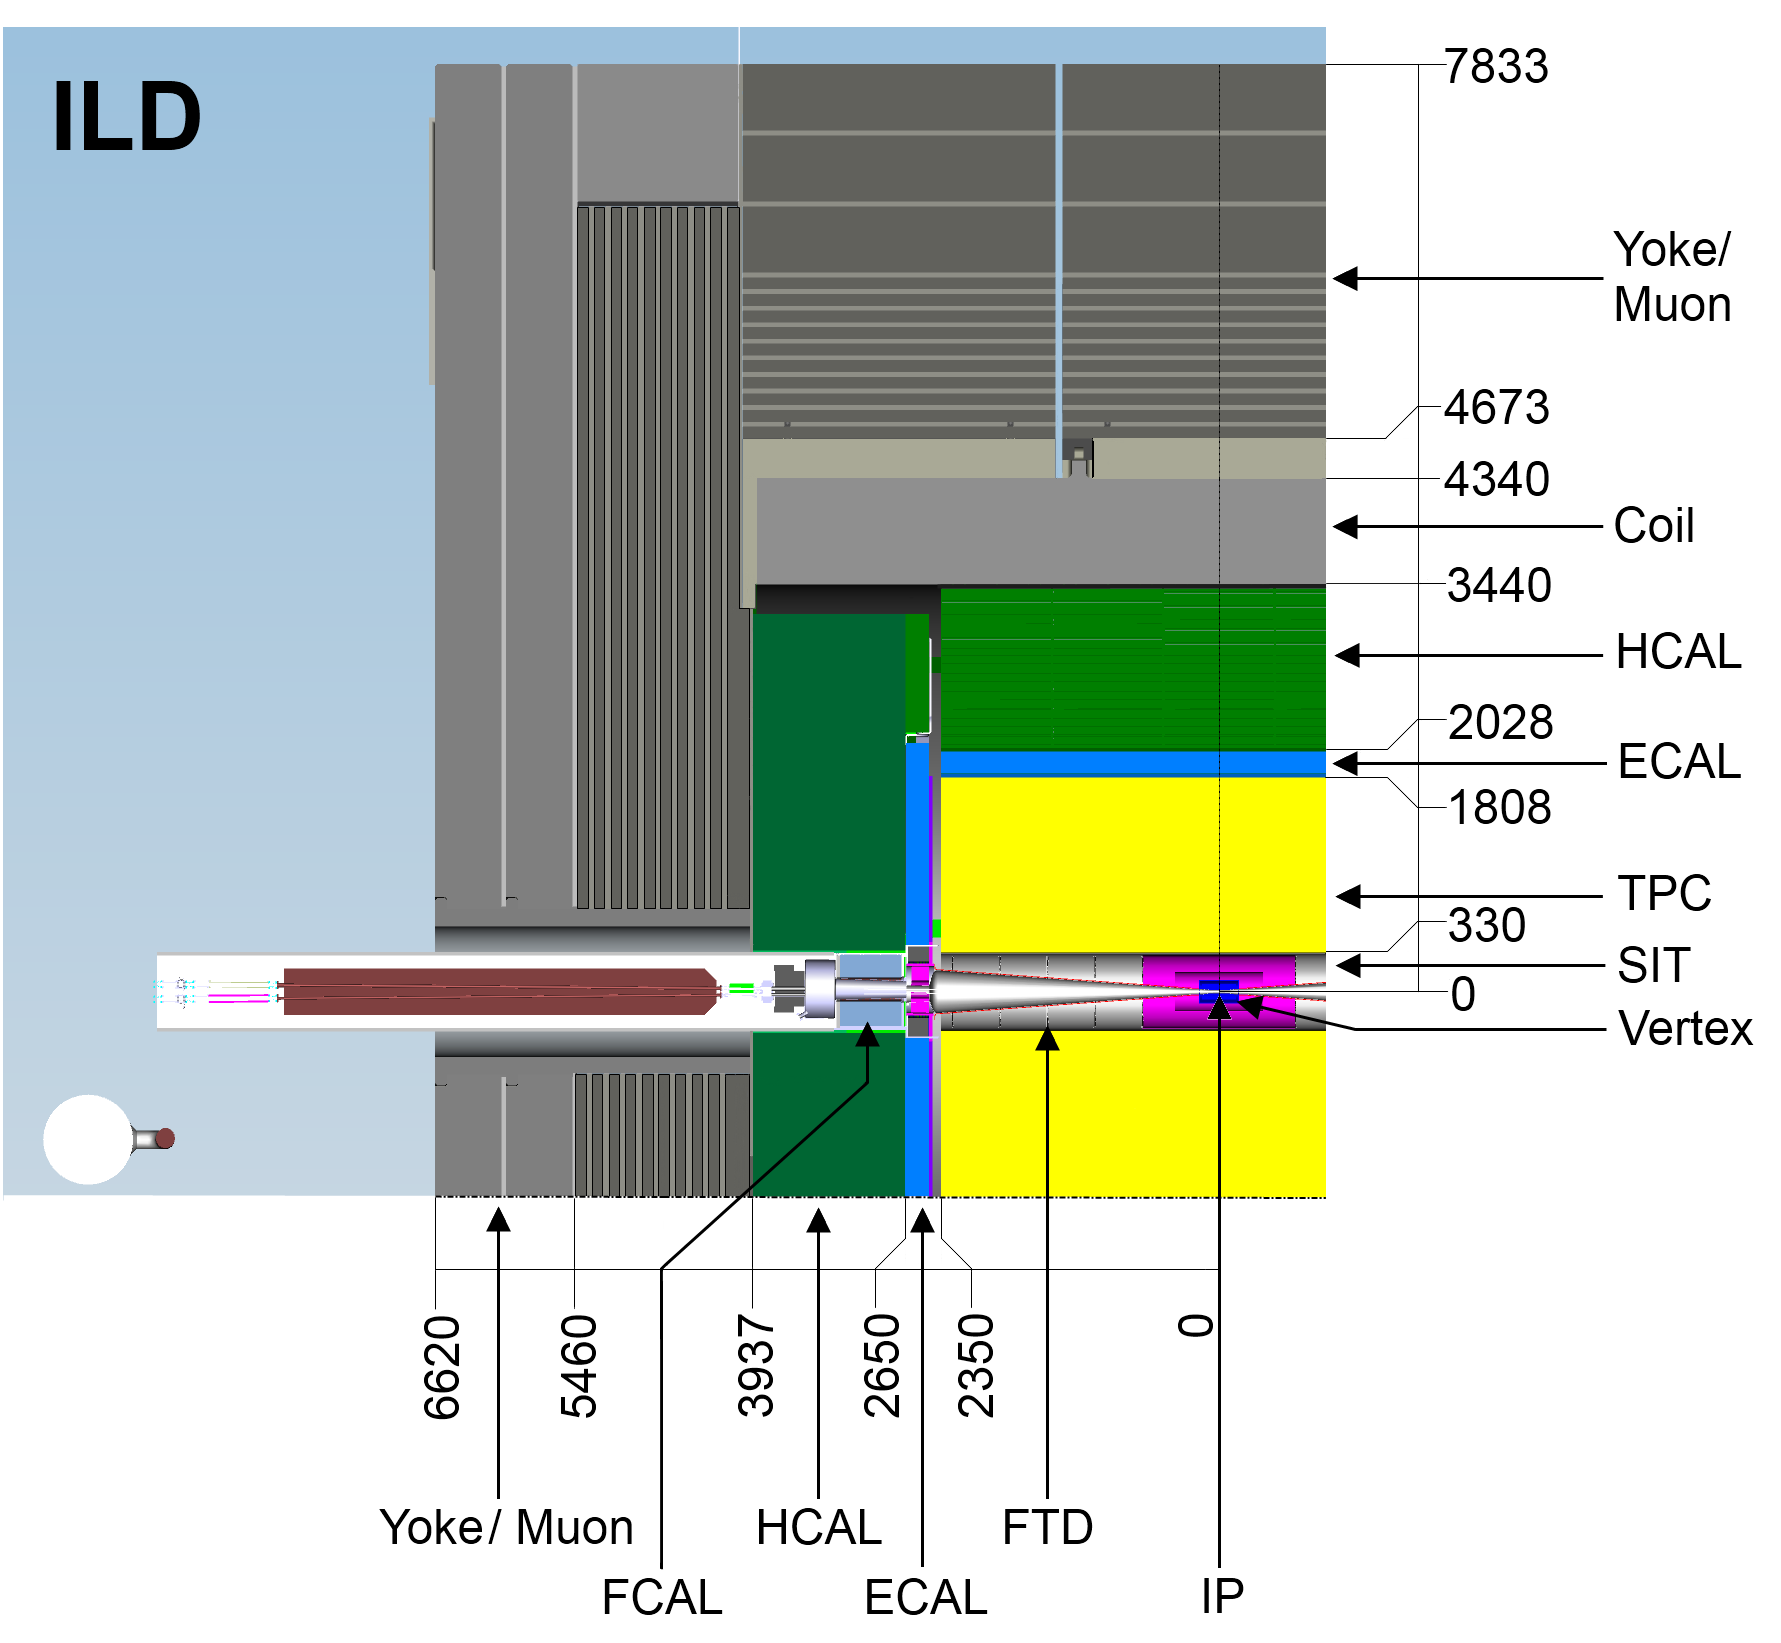
\includegraphics[width=0.8\hsize]{Detector/fig/ILD_quadrant_2.png}
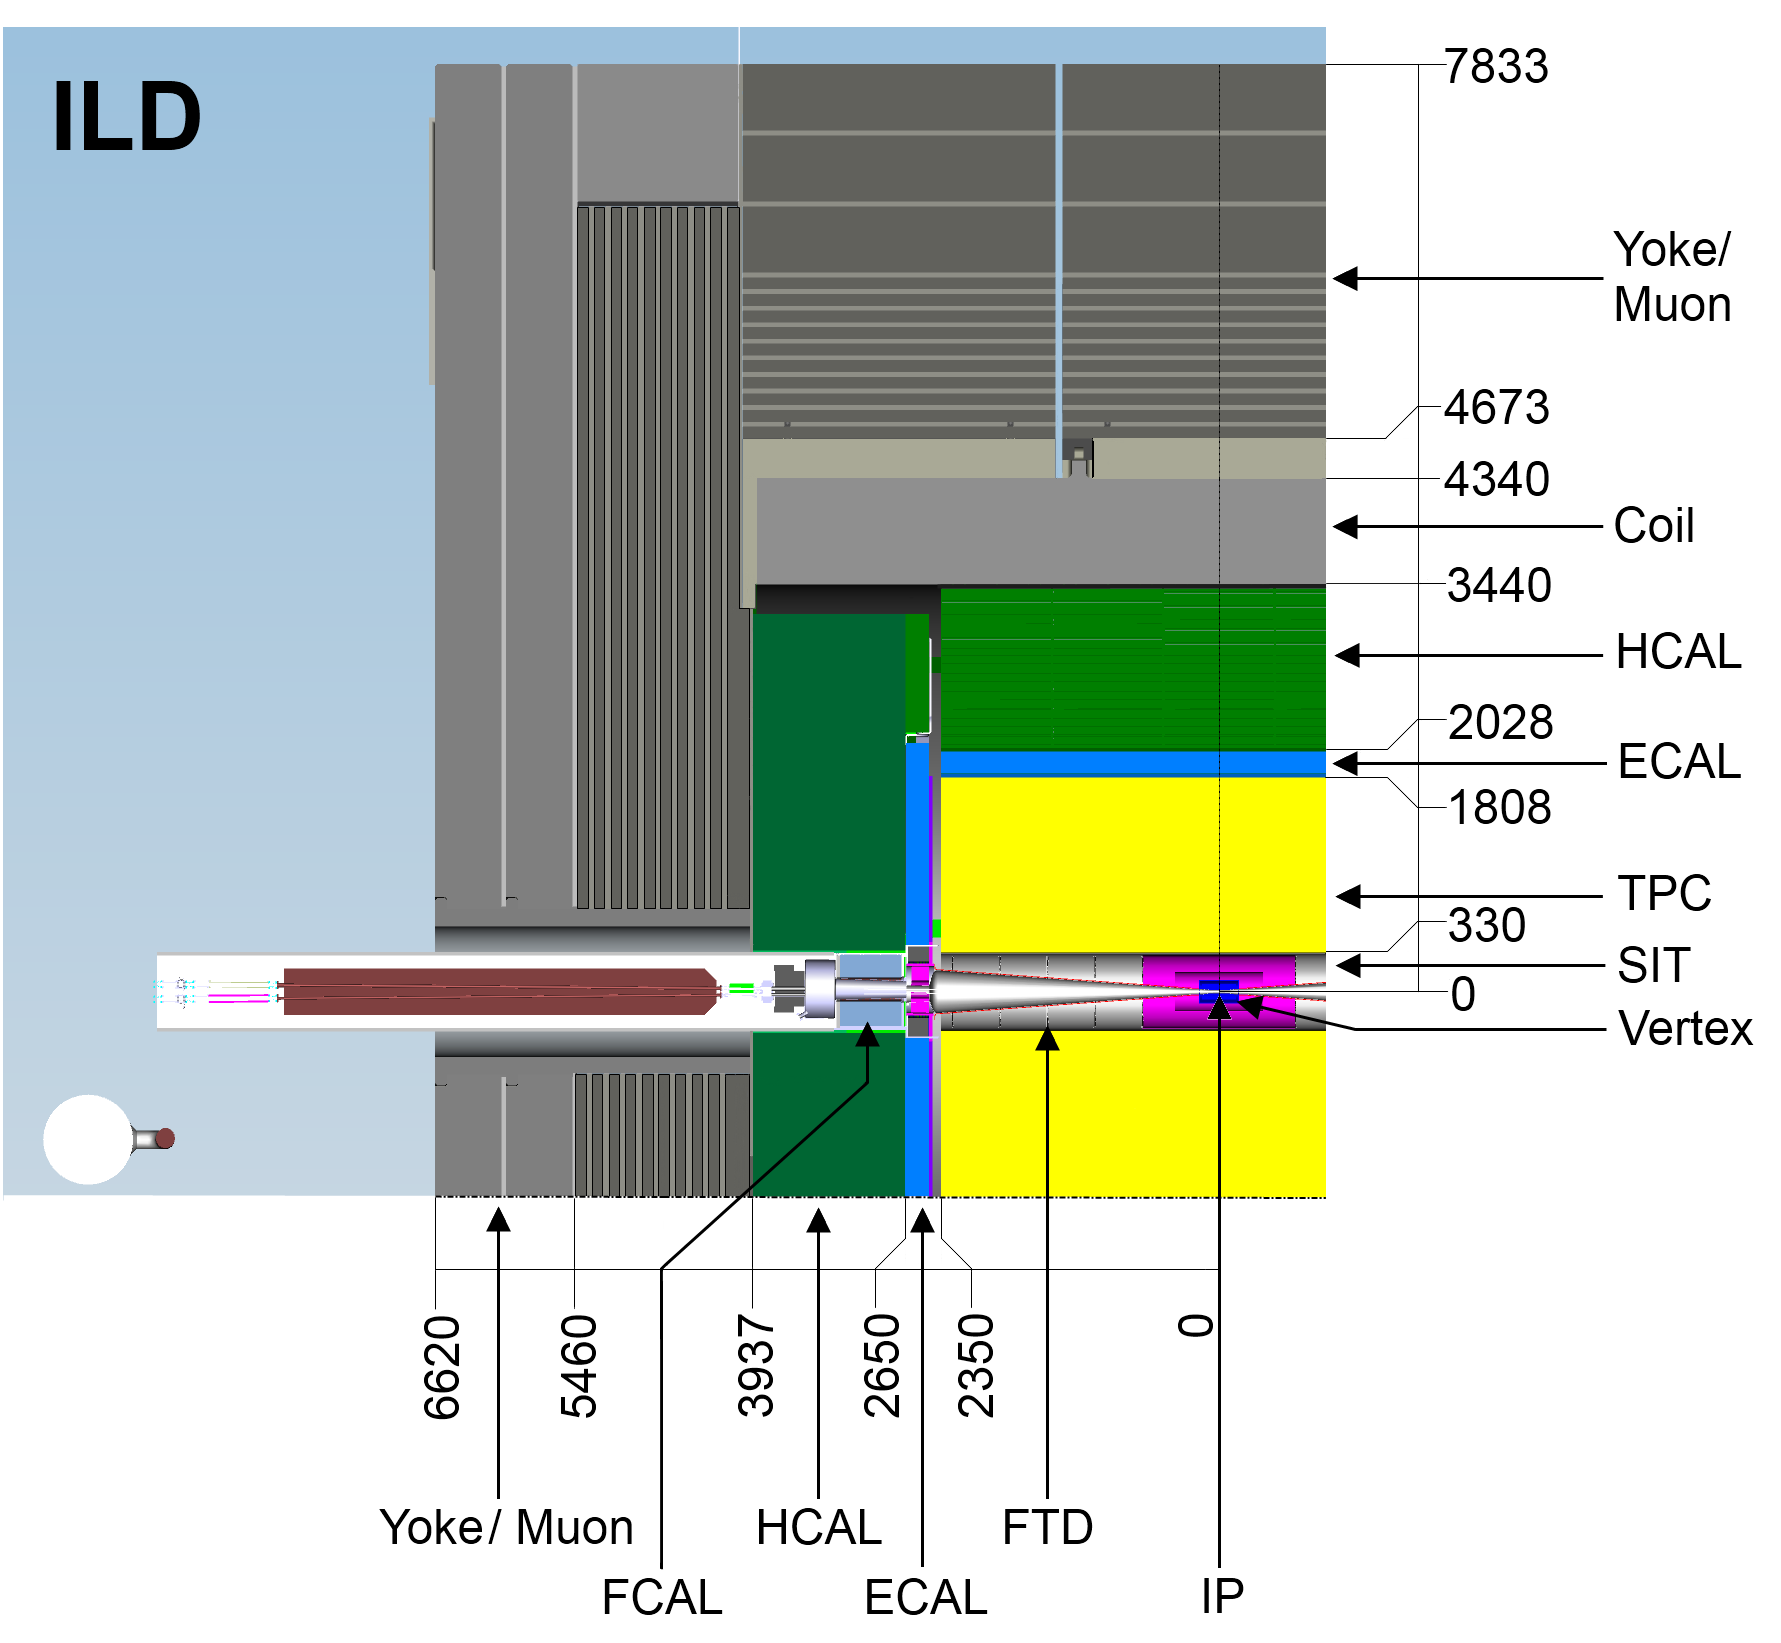
\includegraphics[width=0.6\hsize]{Detector/fig/ILD_quadrant_2.png}
\caption{r-z structure of an ILD quadrant.}
\label{fig:det:quad}
\end{figure}

The overall ILD detector structure is shown in figure ~\ref{fig:det:quad}: a high precision vertex detector positioned very close to the interaction point is followed by a hybrid tracking layout, realised as a combination of silicon tracking with a time projection chamber, and a calorimeter system. The complete system is located inside a large solenoid providing a nominal magnetic field of 3.5T (large ILD) or 4T(small ILD) . On the outside of the coil, the iron return yoke is instrumented as a muon system and as a tail catcher calorimeter. 
The main geometrical parameters are summarised in table~\ref{ild:tab:barrelpara} and table~\ref{ild:tab:endcappara}.
%\begin{sidewaystable}[thb]
\begin{table}\hspace*{-0cm}\small
%\begin{tabular}{|l|p{0.8cm}p{0.8cm}p{1.0cm}|p{2.5cm}p{3.0cm}p{3.0cm}|}
%\begin{tabular}{|l|p{0.06\textwidth}p{0.06\textwidth}p{0.07\textwidth}|p{0.25\textwidth}p{0.20\textwidth}p{0.20\textwidth}|}
\begin{tabular}{ l p{0.05\hsize}p{0.04\hsize}p{0.04\hsize} p{0.20\hsize}p{0.20\hsize}p{0.20\hsize} }
%\hline
\toprule
\multicolumn{7}{l}{{\bf Barrel system}}\\
%\hline
\midrule
System & R(in) & R(out) & z & \multicolumn{3}{l}{comments}\\
       & \multicolumn{3}{c}{[mm]}   &&&\\
%\hline
\midrule
VTX    & 16         & 60        & 125 & 3 double layers &  Silicon pixel sensors, & \\
       &            &           &           & layer 1: & layer 2: & layer 3-6 \\
       &            &           &           & $\sigma<3 \mu m$ & $\sigma < 6 \mu m$ & $\sigma < 4 \mu m$ \\
Silicon &           &           & &&&\\
- SIT   & 153       & 300       & 644   & 2 silicon strip layers & $\sigma = 7 \mu m$& \\
- SET   & 1811      &           & 2300   & 2 silicon strip layers & $\sigma = 7 \mu m$& \\
- TPC   & 330       & 1808      & 2350   & MPGD readout & $1 \times 6 $mm$^2$ pads & $\sigma=60 \mu m$ at zero drift \\
%\hline
\midrule
ECAL    & 1843      & 2028      & 2350   & W absorber  & SiECAL & 30 Silicon sensor layers, $5 \times 5$ mm$^2$ cells \\
        &           &           &        &             & ScECAL & 30 Scintillator layers,  $ 5\times 45$ mm$^2$ strips \\
HCAL    & 2058      & 3410      & 2350   & Fe absorber & AHCAL & 48 Scintillator layers, $3 \times 3$cm$^2$ cells, analogue \\
        &           &           &         &            & SDHCAL & 48 Gas RPC layers, $1\times 1$ cm$^2$ cells, semi-digital\\
%\hline
\midrule
Coil    & 3440      & 4400      & 3950    & 3.5 T field & $ 2 \lambda $& \\
Muon    & 4450      & 7755      & 2800    & 14 scintillator layers& &\\
%\hline
\bottomrule
\end{tabular}
\caption{\label{ild:tab:barrelpara}List of the main parameters of the ILD detector for the barrel part.}
\end{table}

\begin{table}\hspace*{-0cm}\small
%\begin{tabular}{|l|p{0.8cm}p{0.8cm}p{1.0cm}|p{2.5cm}p{3.0cm}p{3.0cm}|}
\begin{tabular}{ l p{0.05\hsize}p{0.04\hsize}p{0.04\hsize} p{0.20\hsize}p{0.20\hsize}p{0.20\hsize} }

%\hline
\toprule
\multicolumn{7}{ l }{{\bf End cap system}}\\
\midrule
System & z(min) & z(max) & r(min), r(max) & \multicolumn{3}{l}{comments}\\
       & \multicolumn{3}{c}{[mm]}   &&&\\
\midrule

FTD    & 220     & 371    &      & 2 pixel disks & $\sigma=2-6 \mu m$ &\\
       &         &        &      & 5 strip disks & $\sigma = 7 \mu m$& \\
ETD    & 2420    & 2445   & 419-1822 & 2 silicon strip layers & $\sigma=7 \mu m$ & \\
\midrule
ECAL   & 2450    & 2635   &      & W-absorber & SiECAL & Si readout layers \\
       &         &        &      &            & ScECAL & Scintillator layers \\
HCAL   & 2650    & 3937   & 335-3190& Fe absorber & AHCAL & 48 Scintillator layers $3 \times 3 $cm$^2$ cells, analogue\\
       &         &        &      &              & SDHCAL & 48 gas RPC layers $1\times 1$cm$^2$ cells, semi-digital \\
BeamCal & 3595   & 3715   & 20-150  & W absorber& 30 GaAs readout layers & \\
Lumical & 2500   & 2634   & 76-280 & W absorber & 30 Silicon layers & \\
LHCAL   & 2680   & 3205   & 93-331 & W absorber &&\\
\midrule
Muon    & 2560   &        & 300-7755 & 12 scintillator layers&&\\
\bottomrule
\end{tabular}
\caption{\label{ild:tab:endcappara}List of the main parameters of the ILD detector for the end cap part.}

\end{table}

A key characteristics of the detector is the amount of material crossed by the particles: particle flow requires a thin tracker to minimise interactions before the calorimeters, and thick calorimeters to fully absorb the showers and measure neutral hadrons. Figure~\ref{fig:det:material} shows the amount of radiation lengths of the trackers material and the total interaction lengths including the calorimeter system. 

\thisfloatsetup{floatwidth=\SfigwFull,capposition=beside}
\begin{figure}[t!]
\begin{tabular}{cc}
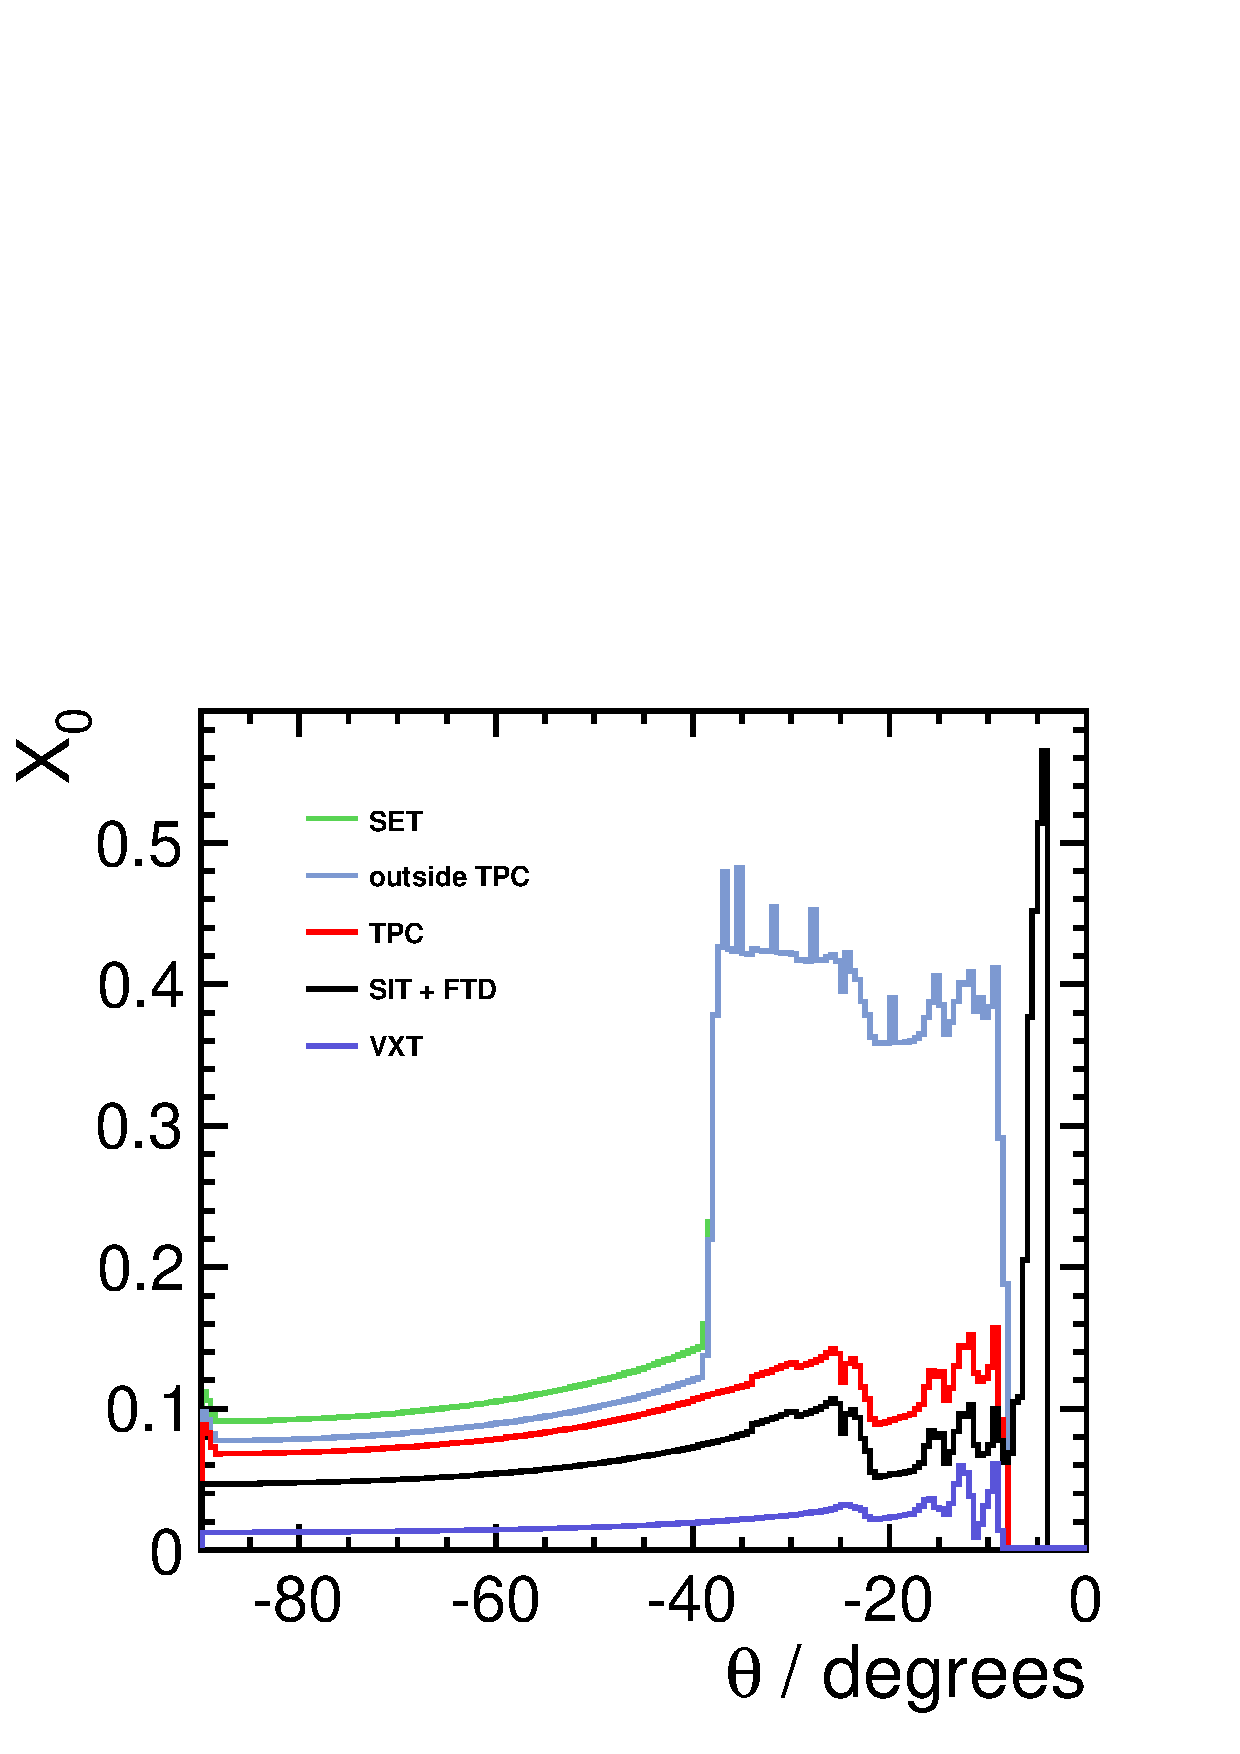
\includegraphics[width=0.52\hsize,viewport={0 -10 600 500},clip]{Detector/fig/material-budget-new.pdf} &
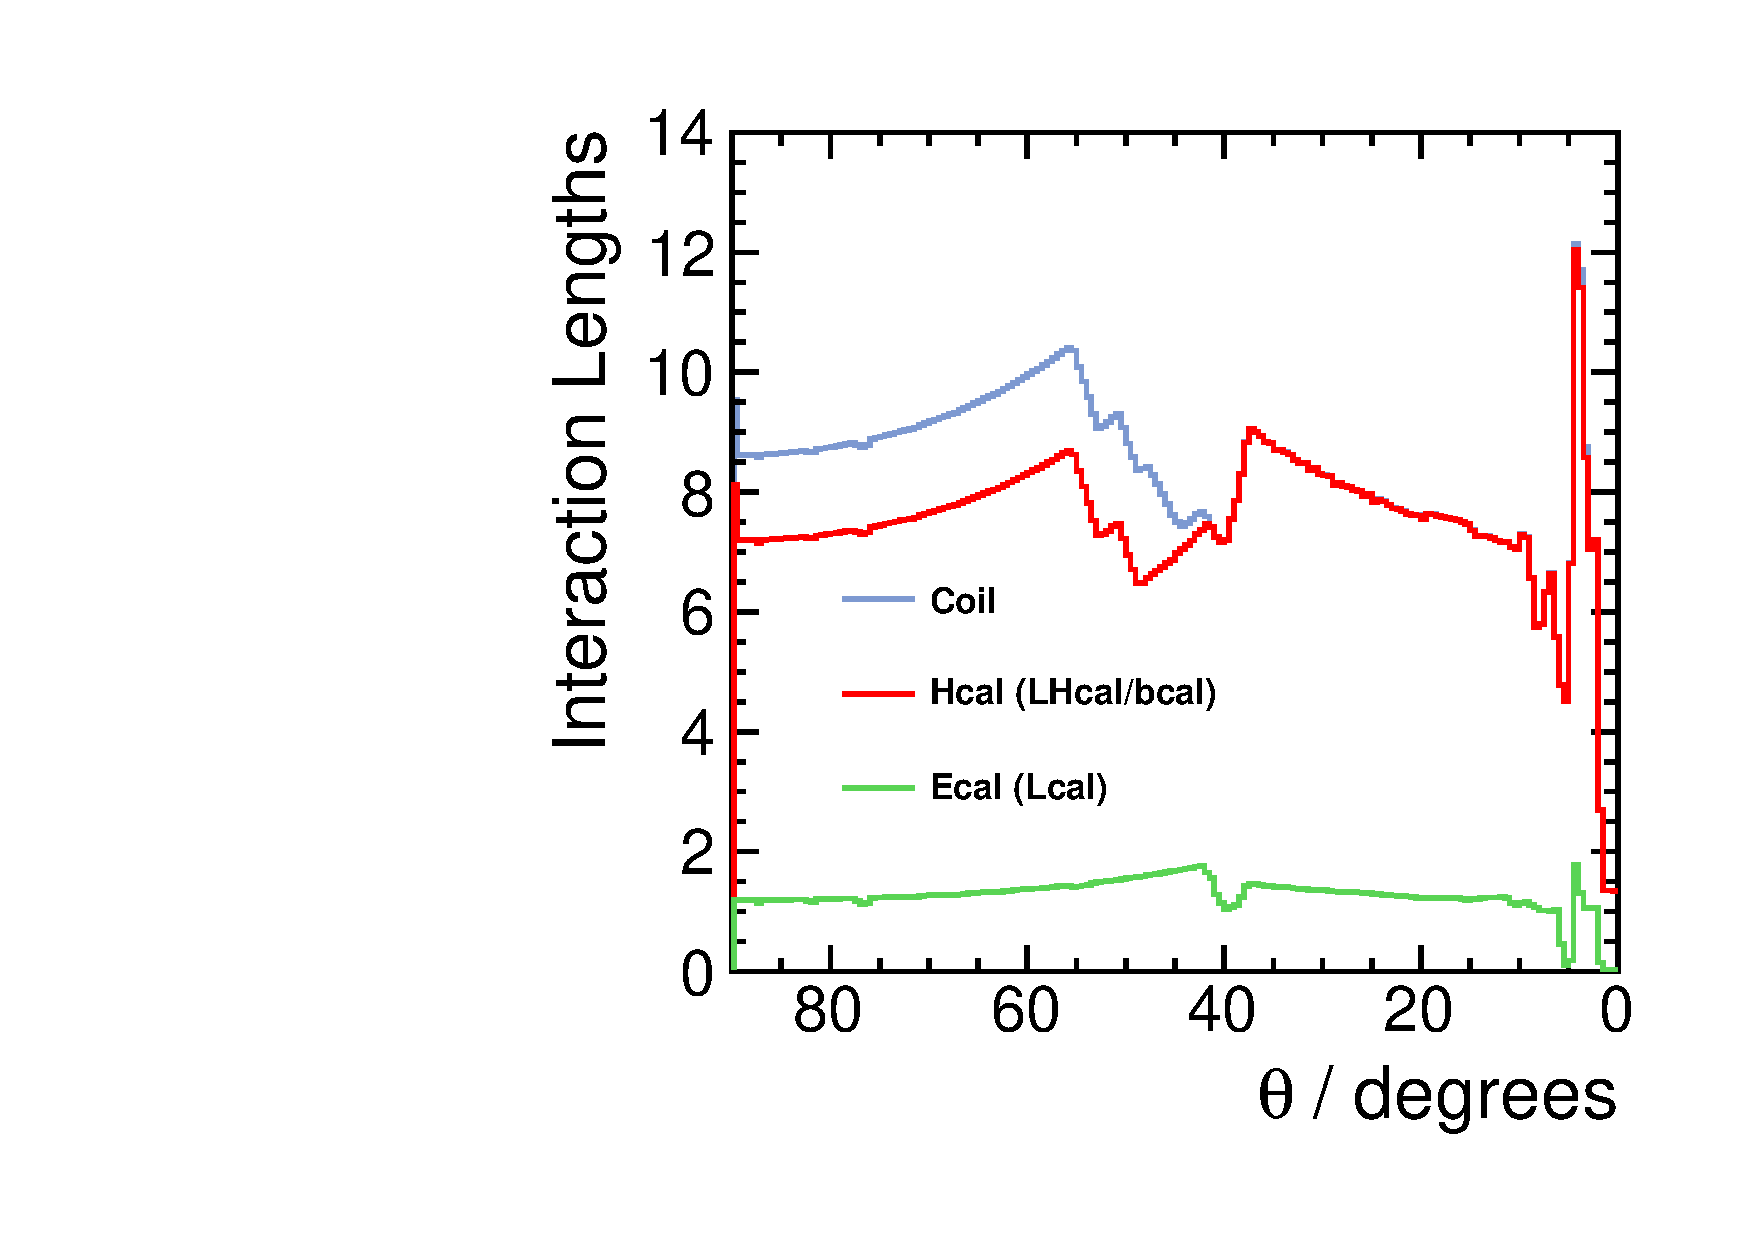
\includegraphics[width=0.5\hsize]{Detector/fig/intlen_ILD_o1_v05.pdf}
\end{tabular}
\caption[Material in the ILD detector]{Left: Average total radiation length of the trackers material as a function of polar angle. Right: Total interaction length seen up to the end of the electromagnetic calorimeter, the hadronic calorimeter and the solenoid coil, respectively.}
%\end{figure}
\label{fig:det:material}
%\begin{tabular}{cc}

\end{figure}

\vspace{2cm}
\subsection{Subdetector layouts}
\writer{Subdetector technical conveners}{4}

The current baseline design of subdetectors is presented including open options. The potential advantages and drawbacks of the various technologies under consideration are discussed together with prospects for enhanced capabilities in the future. The most recent progress and status of each technology will be summarized in section 5.2.

\vspace{1cm}
\subparagraph*{\bf Vertex detector}
\textit{(Besson, Ishikawa, Vos)}

The vertex detector (VTX, Figure~\ref{fig:det:vertex}) is realised as a multi-layer pixel detector with three double-layers. The detector has a pure barrel geometry. To minimise the occupancy from background hits,
the first double-layer is only half as long as the outer two. 



\begin{figure}[t!]
\centering
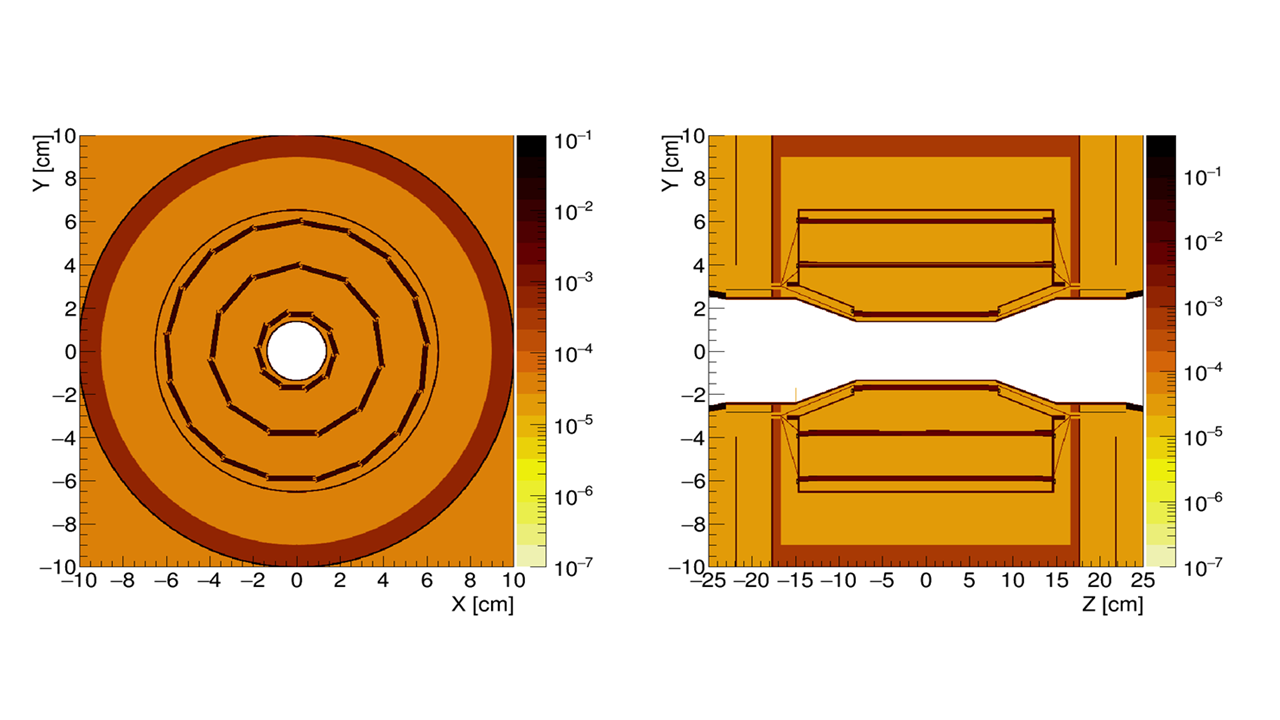
\includegraphics[width=0.6\hsize]{Detector/fig/vertex.png}
\caption{layout of the vertex detector.}
\label{fig:det:vertex}
\end{figure}

Critical parameters of the VTX optimisation are the point resolution for secondary vertex tagging and the material thickness for minimal multiple scattering. Three main technologies are under consideration to achieve the required goals:
\begin{itemize}
    \item {\bf CMOS pixels:} this well-established technology offers the advantages of high granularity with fully monolythic pixel digital electronics available from industrial processes. The most critical points of focus of current R\&D are the readout speed for bunch crossing tagging, the power consumption and the overall material budget of the layers.
    \item {\bf DEPFET pixels:} this technology offers the advantage of high granularity with a small layer material thickness, the digital electronics being shifted at the end of the ladders. Critical aspects are the industrialisation of the fabrication process and the integration of large detector surfaces.
    \item{\bf Fine Pixel CCD (FP-CCD):} CCD's offer the prospects for the highest granularities associated with low power consumption. Another advantage is the minimal material budget of the detector layer, however counter-balanced by the need of a cryostat to ensure low-temperature operation. Critical aspects under study are the readout speed and the resistance to radiation.  
\end{itemize}

\vspace{0.5cm}
The CMOS and DEPFET pixels have typical sizes of 20 microns and are readout in a continuous mode during bunch trains. The readout speed determines the capability to resolve individual bunches. The FPCCD pixels accumulate hits during one bunch train before readout and reset in between trains. Their occupancy is kept acceptable thanks to a smaller pixel size of order 5 microns.  


\vspace{1cm}
\subparagraph*{\bf Silicon trackers}
\textit{(Besson, Vos, Vila)}

A system of silicon trackers surrounds the VTX detector. In the barrel, two layers of silicon detectors (SIT) are arranged to bridge the gap between the VTX and the TPC, and one silicon outer layer (SET) is foreseen inbetween the TPC and the ECAL. In the forward region, a system of seven silicon disks (FTD) provides low angle tracking coverage (Figure~\ref{fig:det:FTD}).

\begin{figure}[t!]
\centering
%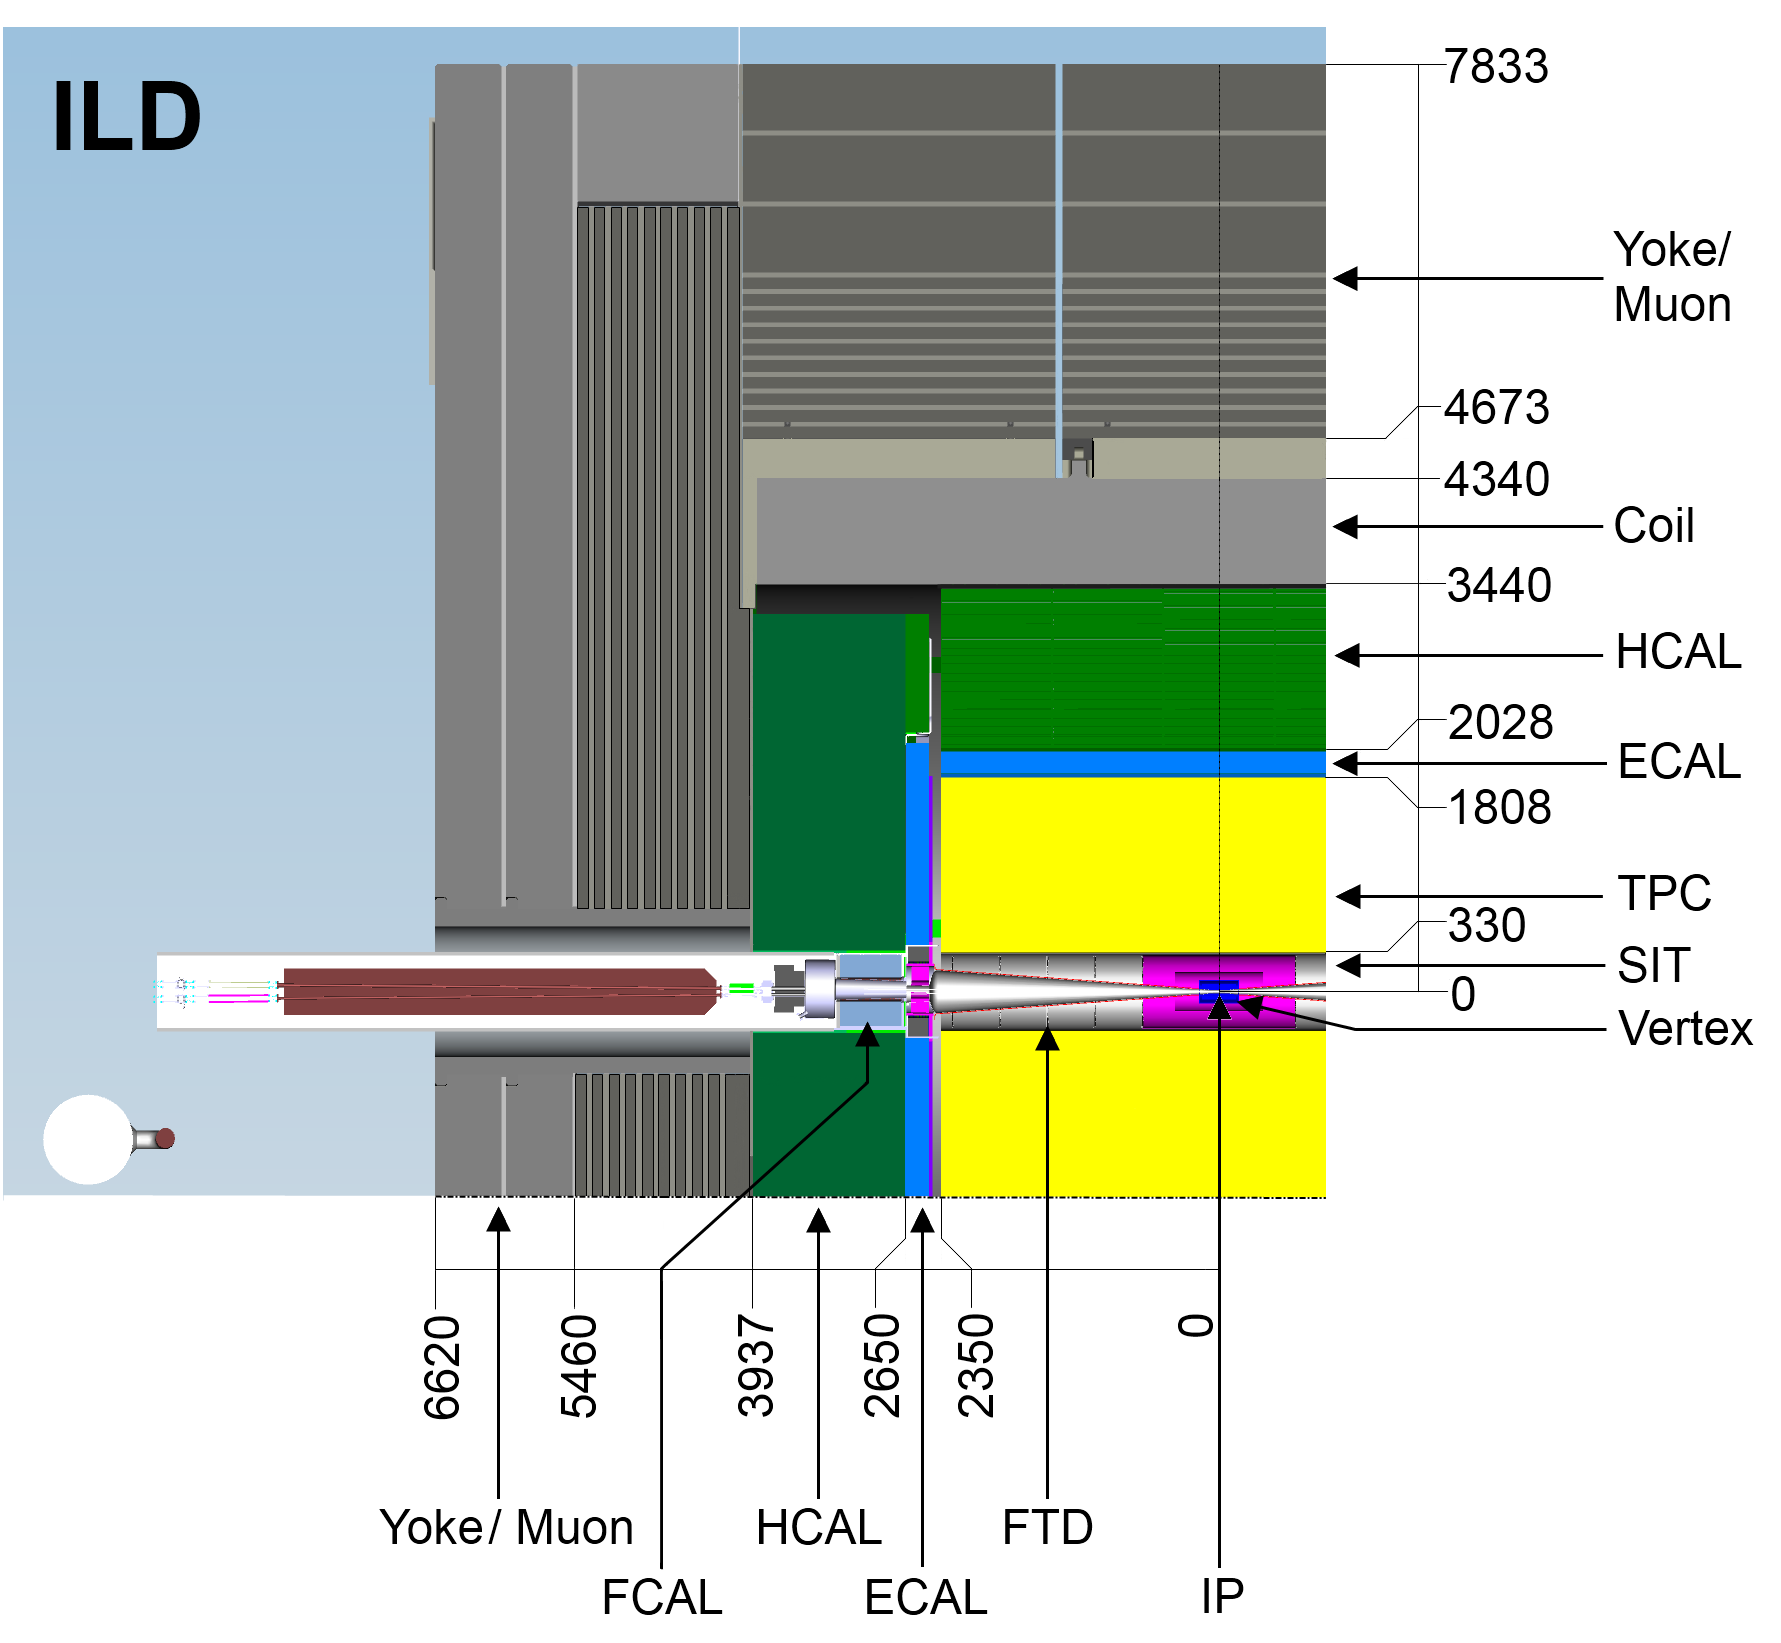
\includegraphics[width=0.8\hsize]{Detector/fig/ILD_quadrant_2.png}
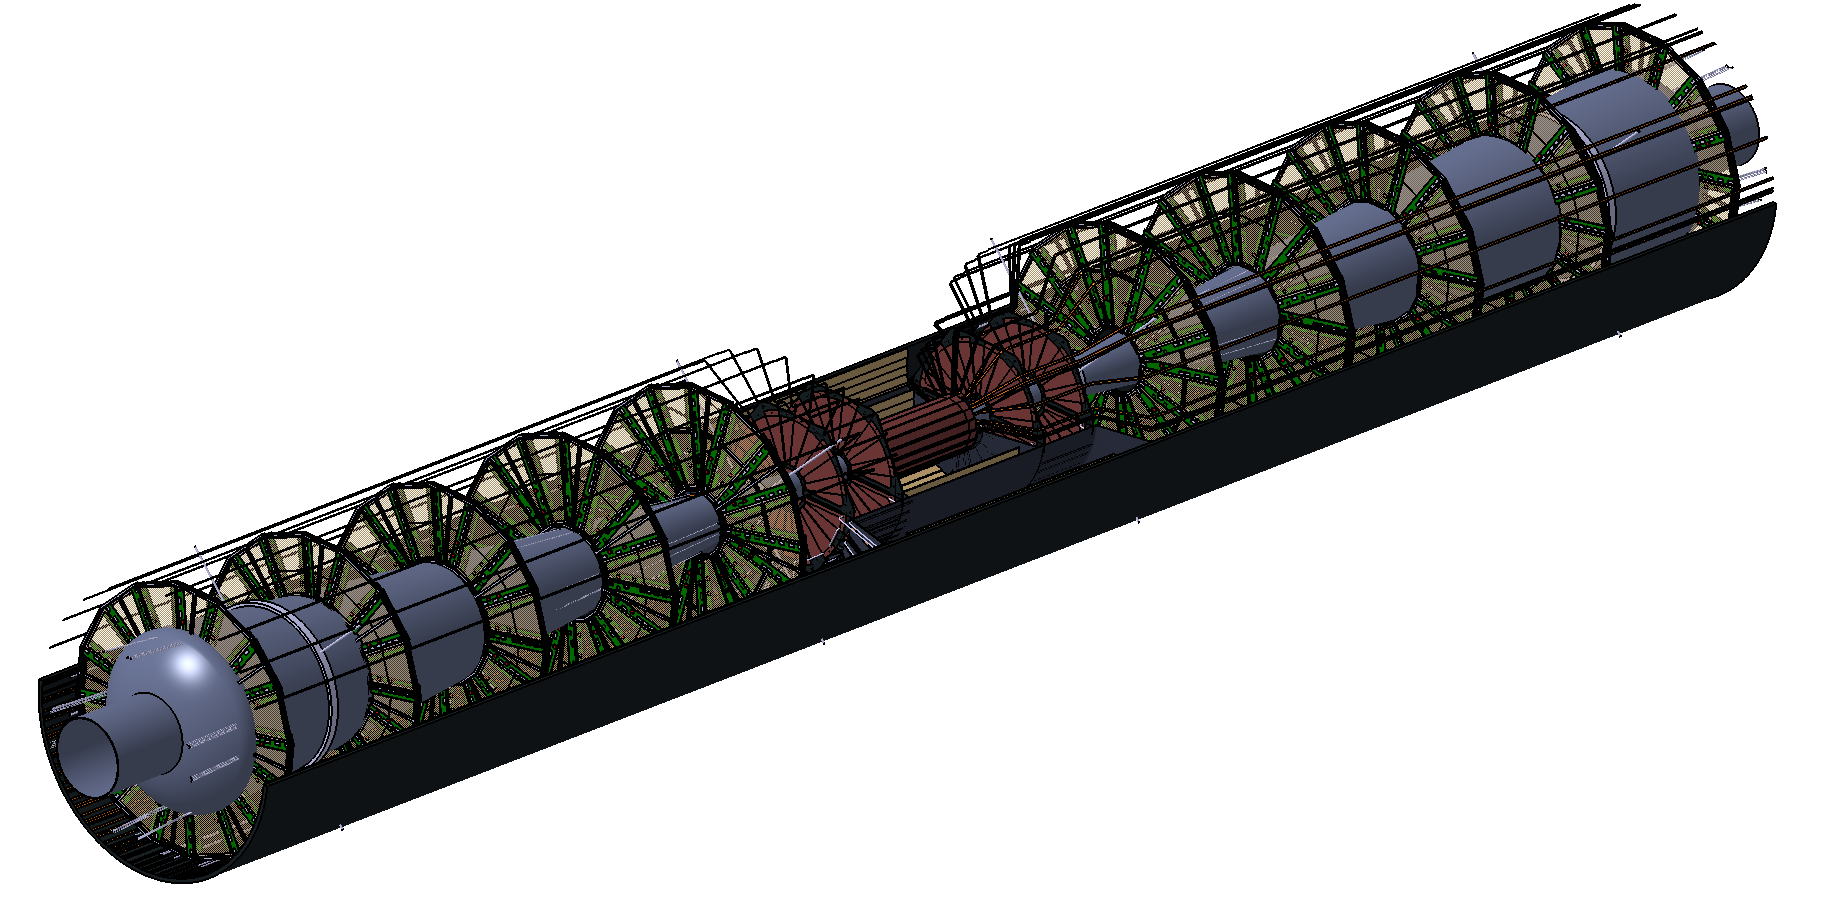
\includegraphics[width=0.6\hsize]{Detector/fig/FTD.png}
\caption{layout of the Forward Tracking Detector.}
\label{fig:det:FTD}
\end{figure}

The baseline technology for the large area trackers is silicon strips but it is considered to move to pixel wherever possible: pixels are already the baseline for the two inner FTD disks, for which the current choice is DEPFET pixels. The possibility to equip more FTD disks with pixels is under study to improve track reconstruction efficiency in the forward region. The progress made with CMOS detectors may also allow to equip the SIT with pixels instead of strips. The design of the SET is still open including the option to implement it as the first layer of the ECAL Calorimeter. The use of high resolution timing detectors is considered in order to provide a TOF functionality for particle identification.   

\vspace{1cm}
\subparagraph*{\bf TPC}
\textit{(Colas, Sugiyama)}

A distinct feature of ILD is a large volume time projection chamber (Figure~\ref{fig:det:TPC} left). The TPC advantages are 3-dimensional point resolution, d$E$/d$x$ based particle identification and minimum material in the field cage. One critical issue concerns potential field distorsions due to ion accumulation within the chamber. At ILC this can be mitigated by implementating an ion gating between bunch trains: ions produced in the gas amplication region during bunch trains are confined and eliminated outside bunch trains by reverting the electric field configuration. This can be implemented with GEM foils as shown in Figure~\ref{fig:det:TPC} right.

%\thisfloatsetup{floatwidth=\SfigwFull,capposition=beside}
\begin{figure}[t!]
\begin{tabular}{cc}
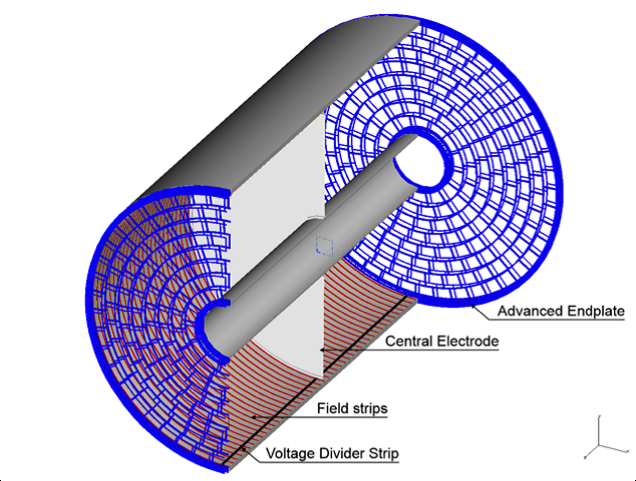
\includegraphics[width=0.6\hsize,viewport={0 -10 600 500},clip]{Detector/fig/TPC.png} &
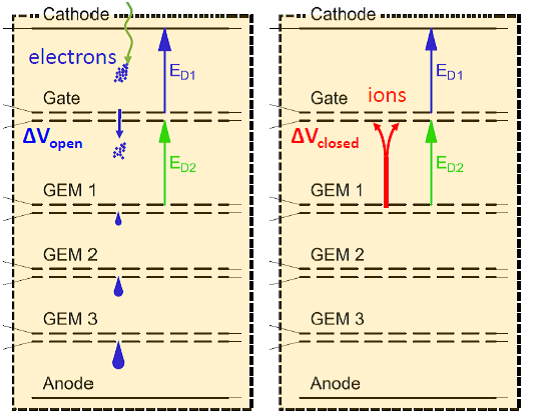
\includegraphics[width=0.4\hsize]{Detector/fig/gating.png}
\end{tabular}
\caption[TPC layout]{Left: Glogal layout of the TPC chamber. Right: Principle of the ion GEM gating scheme showing the 2 electric field configurations within (left) and outside (right) bunch trains.}
%\end{figure}
\label{fig:det:TPC}
%\begin{tabular}{cc}
\end{figure}

Three options are under consideration for the ionisation signal amplification and readout:
\begin{itemize}
    \item GEM readout (Figure~\ref{fig:det:TPC_readout} left): the ionisation signal is amplified by passing through a GEM foil and is collected on pads.
    \item Micromegas readout (Figure~\ref{fig:det:TPC_readout} right): the ionisation signal is amplified between a mesh and the pad array where it is collected.
    \item GRIDPIX: the ionisation signal is amplified as for the micromegas case but collected on a fine silicon pixel grid providing individual pixel timing.
\end{itemize}
\vspace{0.5cm}
For the GEM and micromegas options, the typical pad sizes are a few mm and spatial resolution is improved by combining the track signals of several adjacent pads. For the GRIDPIX option the pixel size of $\approx$50 microns matches the size of the mesh, providing pixel sensitivity to single ionisation electrons. The spatial resolution is improved and the dE/dx signal measured by counting pixels. 

%\thisfloatsetup{floatwidth=\SfigwFull,capposition=beside}
\begin{figure}[t!]
\begin{tabular}{cc}
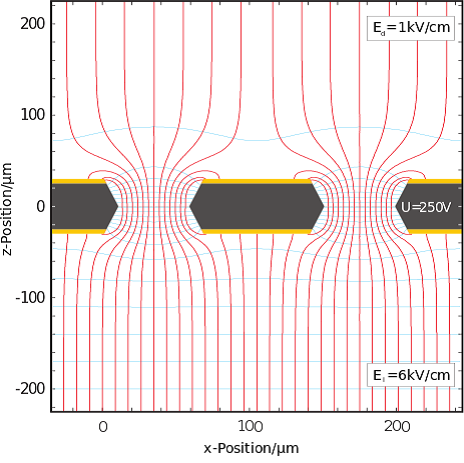
\includegraphics[width=0.5\hsize,viewport={0 -10 600 500},clip]{Detector/fig/GEM.png} &
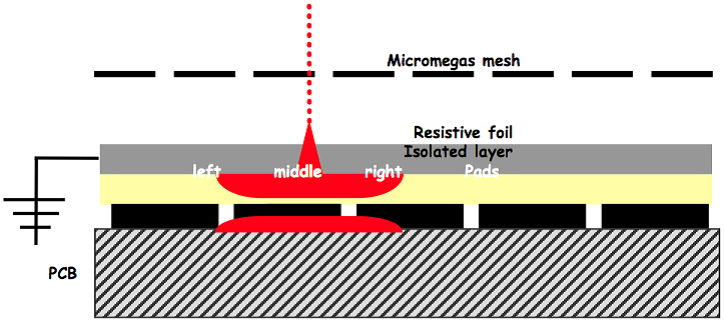
\includegraphics[width=0.4\hsize]{Detector/fig/micromegas.png}
\end{tabular}
\caption[TPC readout]{Amplication scheme of the TPC ionisation signals with GEM (left) and micromegas (right) readout.}
%\end{figure}
\label{fig:det:TPC_readout}
%\begin{tabular}{cc}
\end{figure}

\vspace{1cm}
\subparagraph*{\bf ECAL}
\textit{(Brient, Ootani)}

Electromagnetic showers are measured with a compact highly-segmented calorimeter (Figure~\ref{fig:det:ECAL}) with absorber planes made of tungsten. The ECAL barrel shape is octogonal with individual stacks laid such as to avoid projective dead zones in azimuth. The baseline number of layers is 30, with an option to reduce the number to 22 keeping the amount of radiation lengths identical and increasing the thickness of the sensitive medium to maintain a similar energy resolution.

\begin{figure}[t!]
\centering
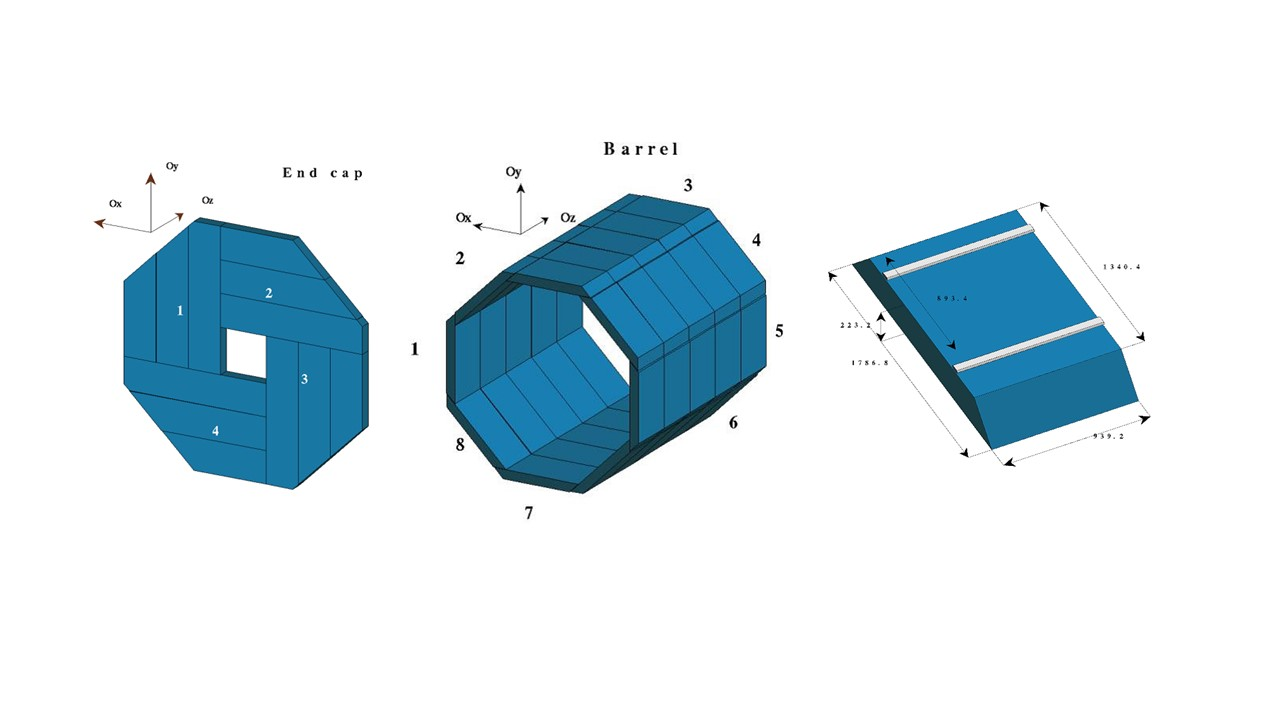
\includegraphics[width=1.2\hsize]{Detector/fig/ECAL_structure.jpg}
\caption{Mechanical structure of the electromagnetic calorimeter: left: endcap wall; center: barrel; right: individual barrel stack.}
\label{fig:det:ECAL}
\end{figure}

The sensitive medium consists in silicon sensors with 5x5 $mm^2$ pads bonded on a PCB equipped with front-end readout ASICs (Figure~\ref{fig:det:ECAL_readout} left). In order to reduce the costs it is also considered to equip part of the sensitive layers with scintillator sensors readout through SiPMs (Figure~\ref{fig:det:ECAL_readout} left). In that case the scintillator strips would have a larger dimension of 30x5$mm^2$ with alternate orthogonal orientation.  

\begin{figure}[t!]
\centering
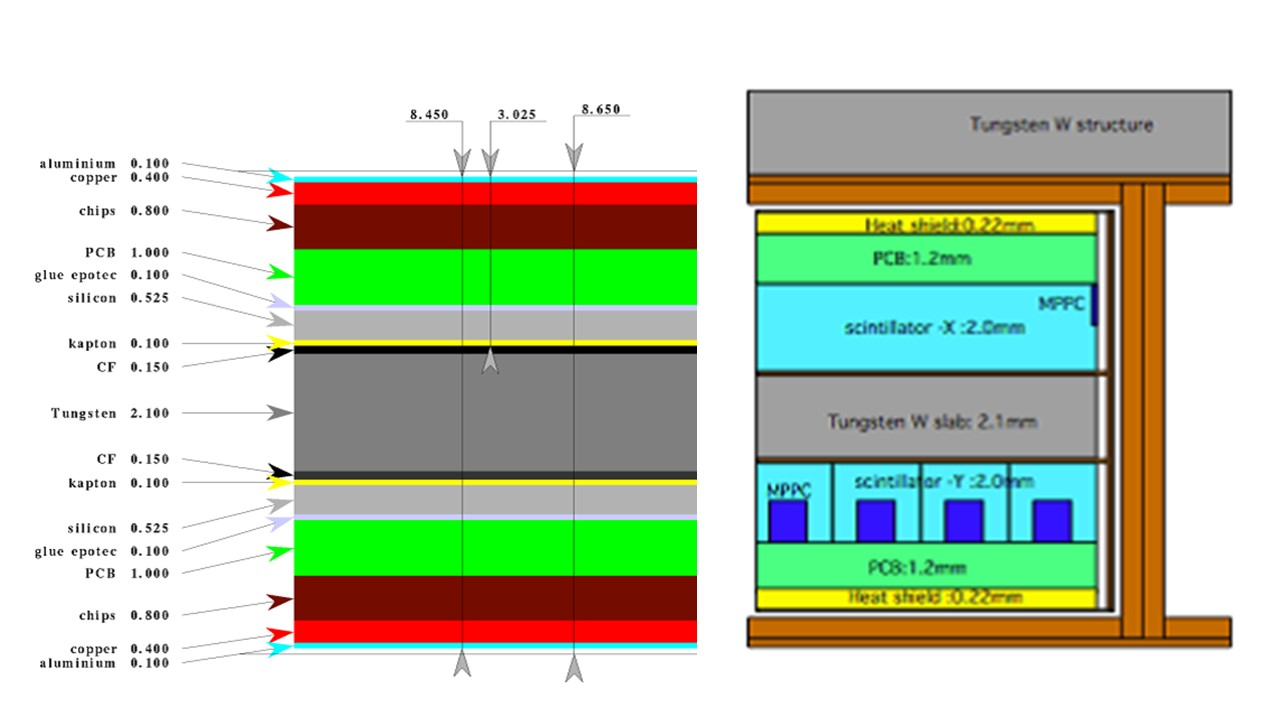
\includegraphics[width=1.0\hsize]{Detector/fig/ECAL_readout.jpg}
\caption{ECAL sensitive layer: left: silicium option; right: scintillator option.}
\label{fig:det:ECAL_readout}
\end{figure}


\vspace{1cm}
\subparagraph*{\bf HCAL}
\textit{(Laktineh, Sefkow)}

The hadronic calorimeter consists in 48 longitudinal samples with steel absorber plates. Two options are currently considered for the mechanical structure, differing mainly in the barrel region (Figure~\ref{fig:det:HCAL}): the "TESLA" barrel made of 2 wheels with signals extracted longitudinally in the gaps between the barrel and endcaps, and the "VIDEAU" barrel made of 3 to 5 wheels with signals extracted at the periphery between the HCAL and coil cryostat. The latter presents no dead zone in azimuth nor at $90^o$ polar angle, and offers a better mechanical stiffness at the cost of a reduced accessibility of the front-end electronics.

\begin{figure}[t!]
\centering
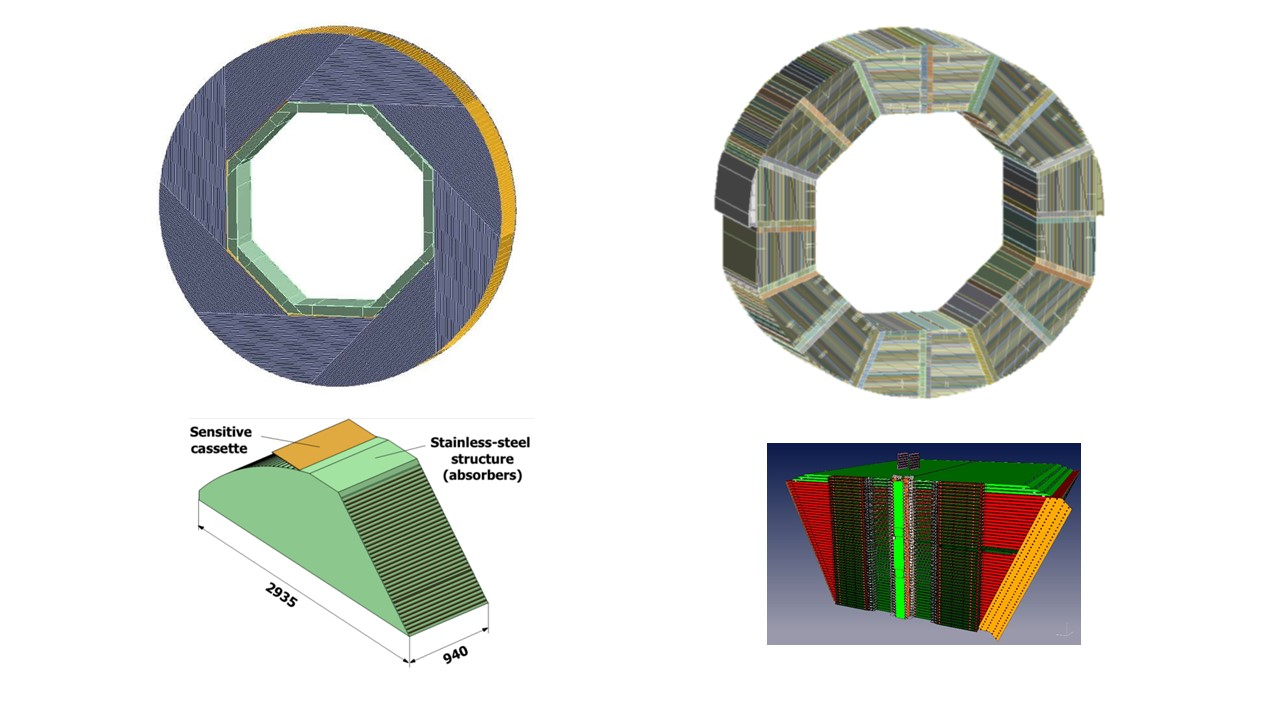
\includegraphics[width=1.1\hsize]{Detector/fig/HCAL_structure.jpg}
\caption{HCAL barrel mechanical structure: full wheel (top) and indiviual stack (bottom) for the two configurations under consideration: the "Videau" option (left) and the "TESLA" option (right).}
\label{fig:det:HCAL}
\end{figure}

The HCAL layers are instrumented with high granularity for an efficient separation of charged and neutral hadronic showers, necessary for particle flow, as well as for a good muon identification for flavor jet tagging. Two sensor options are under consideration (Figure~\ref{fig:det:HCAL_readout}): scintillator tiles of 3x3 $cm^2$ with analog signals readout through SiPMs, and RPC's with pads of 1 $cm^2$ readout with a semi-digital resolution of 2 bits.

\begin{figure}[t!]
\begin{tabular}{cc}
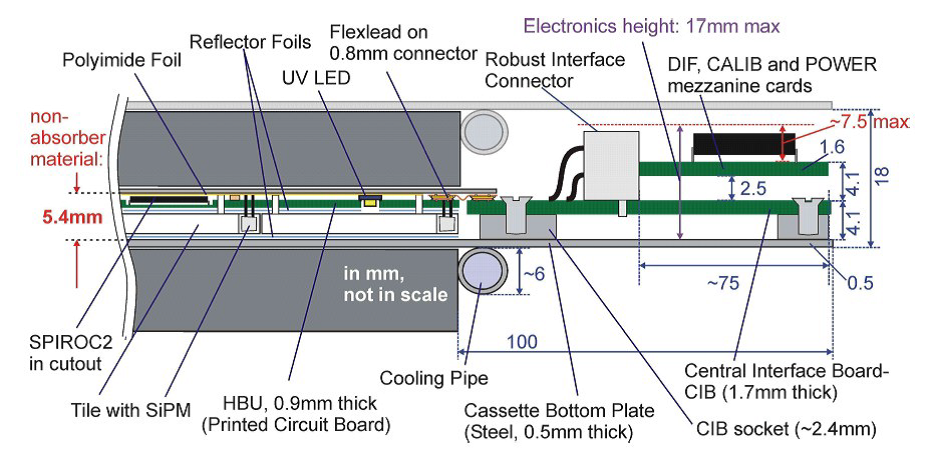
\includegraphics[width=0.5\hsize,viewport={0 -10 600 500},clip]{Detector/fig/AHCAL_layer.png} &
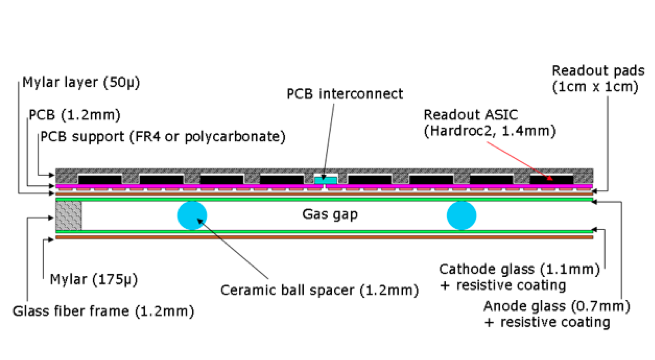
\includegraphics[width=0.5\hsize]{Detector/fig/SDHCAL_layer.png}
\end{tabular}
\caption{HCAL sensitive layer; left: scintillator option; right: RPC option.}
%\end{figure}
\label{fig:det:HCAL_readout}
%\begin{tabular}{cc}
\end{figure}


\vspace{1cm}
\subparagraph*{\bf VFS}
\textit{(Benhammou, Schuwalow)}

The ILD very forward region is equipped with dedicated detectors to perform:
\begin{itemize}
\item a precise determination of the luminosity from Babbha scattering electron pairs (LumiCAL);
\item an extension of the hadronic calorimetry coverage in the forward region (LHCAL);
\item calorimetric hermiticity up to the beam pipe and fast monitoring of beam conditions (BeamCAL).
\end{itemize}
The overal layout of the detectors is shown in Figure~\ref{fig:det:VFS} left. Their longitudinal positioning has been adapted as shown in Figure~\ref{fig:det:VFS} right to account for the new ILC optics (chapter 3).  

%\thisfloatsetup{floatwidth=\SfigwFull,capposition=beside}
\begin{figure}[t!]
\begin{tabular}{cc}
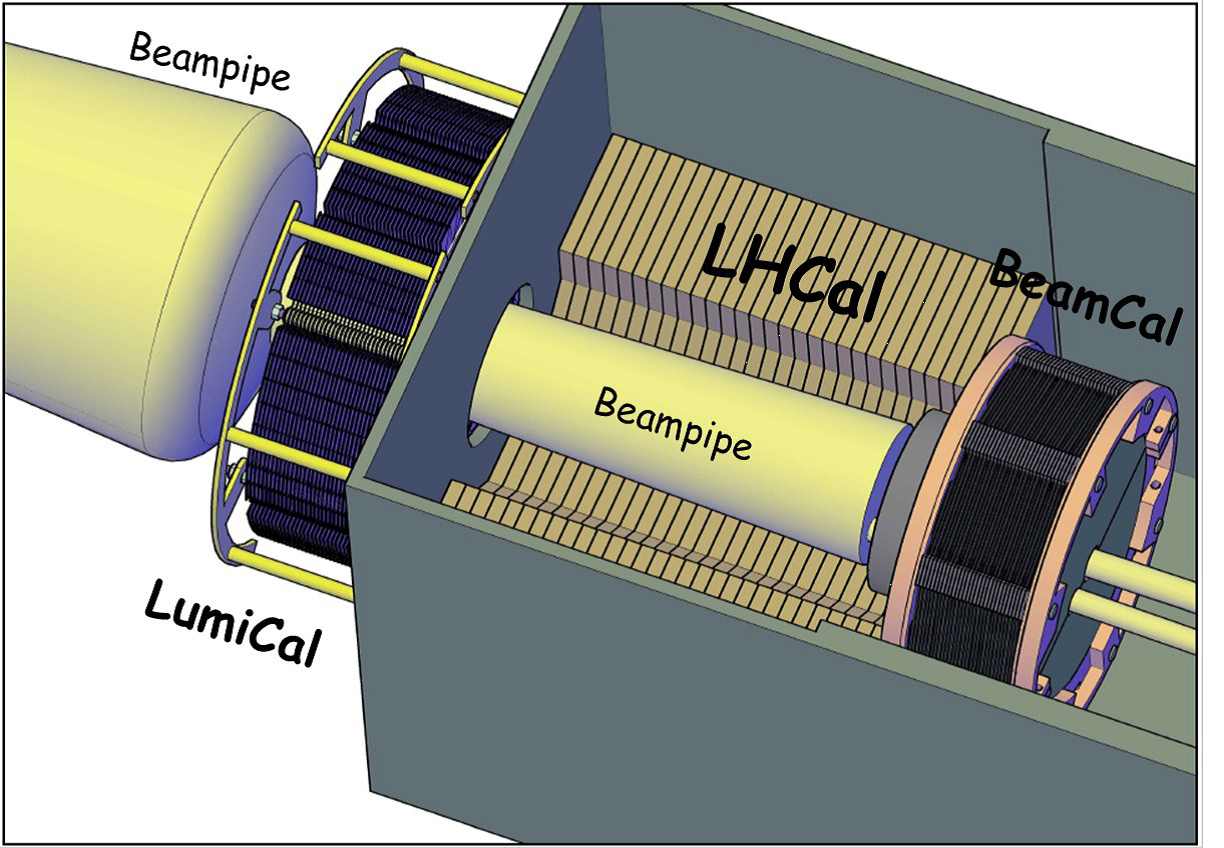
\includegraphics[width=0.5\hsize,viewport={0 -10 600 500},clip]{Detector/fig/VFS_layout.png} &
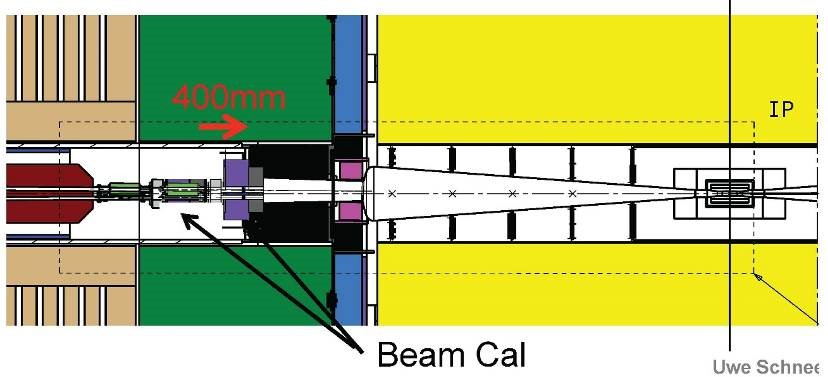
\includegraphics[width=0.4\hsize]{Detector/fig/VFS_newoptics.jpg}
\end{tabular}
\caption{Overall layout of the Very Forward System (left) and adaptations made for the new ILC optics (right).}
%\end{figure}
\label{fig:det:VFS}
%\begin{tabular}{cc}
\end{figure}

\vspace{1cm}
\subparagraph*{\bf Iron instrumentation}
\textit{(Saveliev): sensitive layers in yoke baseline design and sensor structure}

A large volume superconducting coil surrounds the calorimeters, creating an axial $B$-field of nominally 3.5-4\,Tesla.

An iron  yoke, instrumented with scintillator strips or resistive plate chambers (RPCs), returns the magnetic flux of the solenoid, and, at the same time, serves as a muon filter, muon detector and tail catcher calorimeter.

%\vspace{2cm}
\newpage
\section{Subdetector technology status}
\writer{Subdetector conveners}{}

This section is one of the main technical added values of the IDR. It should summarize all technological progress since the DBD, including beam tests of technological prototypes and ongoing spinoffs. It should also indicate the remaining steps to fulfil the ILD requirements, with a focus of critical aspects associated to each technology choice. For conciseness only the highlights should be illustrated, with all details to be referenced in technical publications. As regards illustrations it is proposed to stick to o(1-2) photo and o(1-2) plot  for each technology. 

\vspace{2cm}
\subsection{Vertex detector}
\writer{Auguste Besson, Akimasa Ishikawa, Marcel Vos}{3}

CMOS spin-offs: ALPIDE (ALICE upgrade) and MIMOSIS (CBM), New PSIRA chip for ILD

DEPFET spin-off: BELLE-2, BEAST and first physics events

FPCCD long prototype and irradiation tests

Short mention of other options:  SOI, etc

Low material support developments (PLUME ladder) and cooling studies

\vspace{2cm}
\subsection{Silicon inner tracking detectors}
\writer{Marcel Vos, Ivan Vila}{1}

Above DEPFET developments and FTD thermo-mechanical mockup

\vspace{2cm}
\subsection{Time projection chamber}
\writer{Paul Colas, Akira Sugiyama}{3}

TPC prototype for generic beam tests of all readout options, the gating scheme and cooling. Mention LYCORIS silicon telescope and new field cage in construction.

CO2 Cooling measurements            

Successful gating achieved with GEM

GEM and Micromegas spacial and ionization resolutions

Ongoing technological developments: improved module planarity, GRIDPIX RO options, etc.  

\vspace{2cm}
\subsection{Calorimeters}
\writer{Jean Claude Brient, Wataru Ootani, Felix Sefkow, Imad Laktineh}{5}

Si-ECAL: technological prototype (incl long slab) beamtest results, CMS HGCAL spinoff.

Sc-ECAL results from new detector unit in construction.

AHCAL beamtest results from large technological prototype, CMS HGCAL spinoff.

SDHCAL beamtest results of large technological prototype at CERN, ongoing development of large chambers. 

\vspace{2cm}
\subsection{Very forward detectors}
\writer{Yan Benhammou, Sergej Schuwalow}{2}

LUMICAL sensors: Beam test of thinner prototypes with improved transverse resolution of e-showers

BEAMCAL and LHCAL developments

\vspace{4cm}
\subsection{Iron instrumentation}
\writer{Valery Saveliev}{1}

Fermilab Scintillator detectors prototypes and performance tests

\vspace{2cm}
